
This chapter presents the overall approach for cassava leaf disease classification using deep learning. We outline the pipeline, describe each model evaluated, and present the final proposed framework based on our top-performing architecture.

\section{Method Overview}

Our classification pipeline consists of the following steps:

\begin{enumerate}
    \item \textbf{Data Acquisition:} A publicly available cassava leaf dataset with five classes (four disease types and healthy) is used.
    \item \textbf{Preprocessing:} Images are resized to 224×224 pixels and normalized.
    \item \textbf{Augmentation:} Techniques such as horizontal/vertical flip, random rotation, random crop, and brightness/contrast variation are applied to enhance generalization.
    \item \textbf{Model Selection:} Multiple convolutional neural network (CNN) architectures are evaluated using transfer learning: Xception, EfficientNetB0, ResNet50, VGG16, DenseNet121, InceptionV3, and ReXNet150.
    \item \textbf{Training Setup:} All models are compiled with the Adam optimizer and categorical cross-entropy loss, trained with batch size 32, and monitored using early stopping on validation loss.
    \item \textbf{Evaluation:} Validation accuracy and F1-score guide the selection of the best model.
\end{enumerate}

\section{Models Description}

\begin{itemize}
    \item \textbf{Xception:} Employs depthwise separable convolutions replacing standard Inception modules, improving parameter efficiency.
    \item \textbf{EfficientNetB0:} Uses compound scaling of width, depth, and resolution for an optimal trade-off between accuracy and model size.
    \item \textbf{ResNet50:} Introduces residual connections to allow training of very deep networks by facilitating gradient flow.
    \item \textbf{VGG16:} A classical 16-layer CNN known for its simplicity and uniform architecture of 3×3 convolutions.
    \item \textbf{DenseNet121:} Connects each layer to every other layer in a feed-forward fashion to strengthen feature propagation.
    \item \textbf{InceptionV3:} Utilizes asymmetric convolutions and dimensionality reduction to increase computational efficiency.
    \item \textbf{ReXNet150:} A lightweight, MobileNet-based architecture optimized for efficiency and accuracy. ReXNet150 leverages \textit{depthwise separable convolutions} to reduce computational complexity, splitting standard convolutions into depthwise (per-channel) and pointwise (1x1) operations. It employs \textit{inverted residual blocks} with linear bottlenecks, where input channels are expanded (e.g., 6x), processed with a 3x3 depthwise convolution, and projected back, with skip connections preserving information flow. The architecture progressively increases channel width across stages (e.g., 32 to 1280 channels), enhancing representational capacity with minimal parameter overhead (approximately 10–15 million parameters). With around 150 layers, ReXNet150 stacks multiple blocks in 5–7 stages, each reducing spatial dimensions via strided convolutions. Global average pooling and a fully connected layer produce class predictions. Pre-trained on ImageNet, ReXNet150 adapts well to cassava leaf disease classification, capturing fine-grained features like leaf lesions while maintaining efficiency for potential edge deployment.
\end{itemize}

\section{Proposed Framework}

Based on our comparative evaluation, we select \textbf{ReXNet150} as the core of our final system due to its superior validation accuracy and F1-score, balancing computational efficiency with robust feature extraction. The proposed framework is as follows:

\begin{figure}[H]
  \centering
  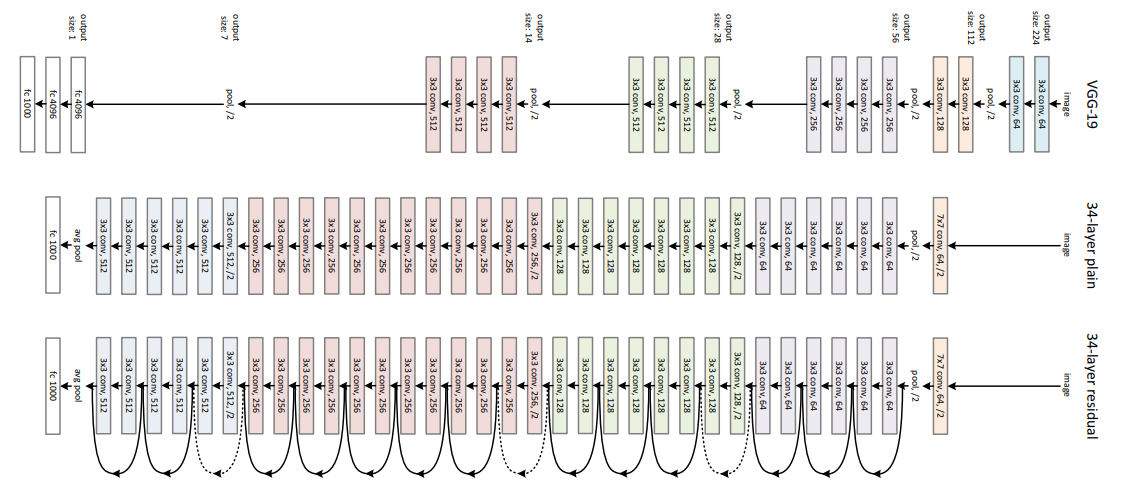
\includegraphics[width=1.0\textwidth]{./figures/ResNet.png}
  \caption{ReXNet150 architecture overview, illustrating the stack of inverted residual blocks with depthwise separable convolutions, progressive channel expansion, and final classifier head.}
  \label{fig:rexnet150_arch}
\end{figure}

\begin{enumerate}
    \item \textbf{Input Layer:} Receive RGB images resized to 224×224.
    \item \textbf{Data Augmentation:}
    \begin{itemize}
      \item Random horizontal/vertical flips
      \item Random rotations (±15°)
      \item Random crops (90–100\% of original area)
      \item Brightness and contrast jitter
    \end{itemize}
    \item \textbf{Feature Extractor:} Pre-trained ReXNet150 (ImageNet weights), with top layers removed. The backbone consists of inverted residual blocks organized in stages, each with depthwise separable convolutions and progressive channel expansion (e.g., 32 to 1280 channels). Skip connections ensure gradient flow, enabling robust feature learning for disease patterns.
    \item \textbf{Global Pooling:} Apply global average pooling to reduce spatial dimensions to a 1x1 feature map, producing a compact feature vector.
    \item \textbf{Classifier Head:}
    \begin{itemize}
      \item Dense layer with 256 units and ReLU activation
      \item Dropout (rate = 0.5) to prevent overfitting
      \item Output dense layer with softmax activation for five-class classification
    \end{itemize}
    \item \textbf{Optimization:}
    \begin{itemize}
      \item Optimizer: Adam
      \item Loss: Categorical Cross-Entropy
      \item Batch size: 32
      \item Learning rate scheduler: ReduceLROnPlateau (reduce by factor 0.1 if validation loss plateaus for 5 epochs)
      \item Early stopping: Halt training if validation loss does not improve for 10 epochs
    \end{itemize}
    \item \textbf{Output:} Predicted probabilities for each of the five classes: Healthy, Cassava Bacterial Blight (CBB), Cassava Brown Streak Disease (CBSD), Cassava Green Mite (CGM), and Cassava Mosaic Disease (CMD).
\end{enumerate}